\documentclass[10pt,letterpaper]{article}
\usepackage[top=0.85in,left=1in,right=1in,footskip=0.75in]{geometry}
\usepackage{amsmath,amssymb}
\usepackage{microtype}
\usepackage{graphicx}
\usepackage{booktabs}
\usepackage{array}
\usepackage{xcolor}
\usepackage[colorlinks=true,allcolors=blue]{hyperref}

\graphicspath{{./}}
\renewcommand{\thefigure}{S\arabic{figure}}
\renewcommand{\thetable}{S\arabic{table}}
\renewcommand{\figurename}{Fig}
\renewcommand{\tablename}{Table}

\title{\vspace*{-0.8in}\Large\textbf{Supplementary Materials: A Four-Dimension Pre-Modeling Audit Protocol for Educational Prediction Benchmarks}}
\author{Yan Ma\textsuperscript{1,3} \and Lizhuo Zhang\textsuperscript{2,*}}
\date{}

\begin{document}
\maketitle
\vspace{-0.4in}
\noindent\textsuperscript{1} School of Education, Hunan Agricultural University, Changsha 410128, China\\
\textsuperscript{2} School of Information and Intelligence, Hunan Agricultural University, Changsha 410128, China\\
\textsuperscript{3} School of Foreign Studies, Changsha University of Science and Technology, Changsha 410114, China\\
\textsuperscript{*} Correspondence: zhanglizhuo@hunau.edu.cn

\vspace{0.2in}

This document contains supplementary tables and figures for the main manuscript.

\section*{S1 Supplementary Table}

\begin{table}[!h]
\centering
\caption{Model-complexity ablation: instability ratio ($I$) and beat rate across linear and nonlinear models on 100 repeated 80/20 splits.}
\label{tab:model_complexity}
\small
\begin{tabular}{l l c c c c c}
\toprule
Dataset & Model & MAE (mean $\pm$ SD) & $R^2$ (mean) & $r$ (mean) & $I$ & Beat rate \\
\midrule
MM-TBA & Linear & $0.795 \pm 0.089$ & $-0.067$ & $0.178$ & $2.21$ & $0.80$ \\
 & Ridge & $0.793 \pm 0.089$ & $-0.061$ & $0.183$ & $2.09$ & $0.81$ \\
 & Random Forest & $0.815 \pm 0.081$ & $-0.063$ & $0.196$ & $3.96$ & $0.65$ \\
 & Gradient Boosting & $0.856 \pm 0.095$ & $-0.227$ & $0.129$ & $4.60$ & $0.45$ \\
\midrule
Higher Ed & Linear & $1.695 \pm 0.199$ & $0.041$ & $0.469$ & $0.90$ & $0.83$ \\
 & Ridge & $1.686 \pm 0.195$ & $0.054$ & $0.470$ & $0.84$ & $0.83$ \\
 & Random Forest & $1.193 \pm 0.130$ & $0.521$ & $0.744$ & $0.18$ & $1.00$ \\
 & Gradient Boosting & $1.273 \pm 0.146$ & $0.464$ & $0.711$ & $0.23$ & $1.00$ \\
\midrule
xAPI-Edu & Linear & $0.363 \pm 0.025$ & $0.614$ & $0.786$ & $0.12$ & $1.00$ \\
 & Ridge & $0.357 \pm 0.023$ & $0.626$ & $0.799$ & $0.11$ & $1.00$ \\
 & Random Forest & $0.308 \pm 0.023$ & $0.682$ & $0.830$ & $0.09$ & $1.00$ \\
 & Gradient Boosting & $0.327 \pm 0.024$ & $0.663$ & $0.818$ & $0.10$ & $1.00$ \\
\midrule
Entrance Exam & Linear & $0.598 \pm 0.033$ & $0.438$ & $0.670$ & $0.12$ & $1.00$ \\
 & Ridge & $0.594 \pm 0.032$ & $0.448$ & $0.676$ & $0.11$ & $1.00$ \\
 & Random Forest & $0.612 \pm 0.036$ & $0.372$ & $0.628$ & $0.14$ & $1.00$ \\
 & Gradient Boosting & $0.595 \pm 0.033$ & $0.442$ & $0.671$ & $0.12$ & $1.00$ \\
\midrule
UCI Student & Linear & $2.011 \pm 0.148$ & $0.242$ & $0.530$ & $0.36$ & $1.00$ \\
 & Ridge & $2.010 \pm 0.148$ & $0.263$ & $0.530$ & $0.36$ & $1.00$ \\
 & Random Forest & $2.005 \pm 0.151$ & $0.285$ & $0.548$ & $0.37$ & $1.00$ \\
 & Gradient Boosting & $2.046 \pm 0.151$ & $0.257$ & $0.531$ & $0.41$ & $1.00$ \\
\midrule
Dropout & Linear & $0.206 \pm 0.006$ & $0.651$ & $0.807$ & $0.021$ & $1.00$ \\
 & Ridge & $0.206 \pm 0.006$ & $0.651$ & $0.807$ & $0.021$ & $1.00$ \\
 & Random Forest & $0.153 \pm 0.006$ & $0.684$ & $0.828$ & $0.019$ & $1.00$ \\
 & Gradient Boosting & $0.160 \pm 0.006$ & $0.692$ & $0.832$ & $0.019$ & $1.00$ \\
\midrule
OULAD & Linear & $0.296 \pm 0.002$ & $0.471$ & $0.687$ & $0.010$ & $1.00$ \\
 & Ridge & $0.296 \pm 0.002$ & $0.471$ & $0.687$ & $0.010$ & $1.00$ \\
 & Random Forest & $0.193 \pm 0.003$ & $0.577$ & $0.761$ & $0.009$ & $1.00$ \\
 & Gradient Boosting & $0.203 \pm 0.002$ & $0.610$ & $0.781$ & $0.008$ & $1.00$ \\
\bottomrule
\end{tabular}
\end{table}

\clearpage
\section*{S2 EDA Summary}

\begin{table}[!h]
\centering
\caption{Exploratory data analysis summary for the seven audited datasets. All releases contain zero missing values. The datasets that fail the audit (MM-TBA, Higher Ed, UCI Student) do not show distinctive EDA red flags---such as extreme imbalance or redundant features---that would pre-emptively disqualify them; the fragility is only revealed through the four-dimension audit.}
\label{tab:eda_summary}
\small
\begin{tabular}{l r r l l r r r}
\toprule
Dataset & $N$ & Feat. & Target & Dist. & $n_{\mathrm{grp}}$ & Grp sz (min/mean/max) \\
\midrule
OULAD & 32,593 & 44 & Pass=1, Fail/W=0 & 0.47:0.53 & 22 & 365/1482/2498 \\
Dropout & 3,630 & 36 & Grad=1, Dropout=0 & 0.61:0.39 & 17 & 9/214/666 \\
Entrance Exam & 666 & 49 & 4-class ordinal & 24\%:32\%:30\%:15\% & 3 & 21/222/396 \\
UCI Student & 649 & 56 & Grade $G3$ [0,20] & $\mu=11.9$, $\sigma=3.2$ & 2 & 226/324/423 \\
xAPI-Edu & 480 & 72 & 3-class ordinal & 26\%:44\%:30\% & 12 & 19/40/95 \\
MM-TBA & 186 & 13 & Lecture quality [0.5,7.5] & $\mu=6.0$, $\sigma=1.0$ & 0 & --- \\
Higher Ed & 145 & 31 & Grade [0,7] & $\mu=3.5$, $\sigma=2.2$ & 9 & 2/16/66 \\
\bottomrule
\end{tabular}
\end{table}

\clearpage
\section*{S3 Train-Test $R^2$ Gap}

\begin{table}[!h]
\centering
\caption{Train-test $R^2$ gap across 100 repeated 80/20 splits using the same preprocessing pipeline as the main audit (pre-standardise, then split). The gap (train $R^2$ -- test $R^2$) quantifies how much of the apparent iid signal is lost on held-out samples from the same distribution. On UCI Student, the linear-model train-test gap (0.105) is small relative to the iid-to-group-holdout collapse (0.242 to $-0.097$), confirming that the group-holdout failure is not attributable to ordinary overfitting. On OULAD, both gaps remain small.}
\label{tab:train_test_gap}
\small
\begin{tabular}{l l r r r r}
\toprule
Dataset & Model & Train $R^2$ mean & Test $R^2$ mean & Gap mean & Gap SD \\
\midrule
UCI Student & Linear & 0.347 & 0.242 & 0.105 & 0.091 \\
 & Ridge & 0.347 & 0.242 & 0.105 & 0.091 \\
 & RF & 0.898 & 0.276 & 0.622 & 0.081 \\
 & GBT & 0.714 & 0.244 & 0.470 & 0.103 \\
\midrule
Higher Ed & Linear & 0.550 & 0.041 & 0.509 & 0.299 \\
 & Ridge & 0.550 & 0.054 & 0.496 & 0.292 \\
 & RF & 0.937 & 0.518 & 0.419 & 0.140 \\
 & GBT & 0.919 & 0.494 & 0.425 & 0.141 \\
\midrule
OULAD & Linear & 0.282 & 0.268 & 0.014 & 0.024 \\
 & Ridge & 0.282 & 0.268 & 0.014 & 0.024 \\
 & RF & 0.912 & 0.376 & 0.536 & 0.024 \\
 & GBT & 0.468 & 0.399 & 0.069 & 0.024 \\
\bottomrule
\end{tabular}
\end{table}

\clearpage
\section*{S4 Group-Holdout Uncertainty}

\begin{table}[!h]
\centering
\caption{Across-group variation in group-holdout $R^2$. The SD quantifies how consistent the group-holdout performance is across held-out groups. For UCI Student (2 schools), the linear-model SD of 0.154 with a narrow range ($-0.206$ to $0.012$) confirms uniform collapse rather than group-specific failure. For OULAD (22 cohorts), the across-cohort SD of 0.166 and full range ($0.041$ to $0.654$) reflect positive---though variable---cross-group generalization.}
\label{tab:group_holdout_uncertainty}
\small
\begin{tabular}{l l r r r r}
\toprule
Dataset & Model & Groups tested & Mean $R^2$ & SD $R^2$ & Min / Max $R^2$ \\
\midrule
UCI Student & Linear & 2 & $-0.097$ & 0.154 & $-0.206$ / 0.012 \\
 & Ridge & 2 & $-0.094$ & 0.151 & $-0.201$ / 0.012 \\
 & RF & 2 & 0.018 & 0.154 & $-0.091$ / 0.127 \\
 & GBT & 2 & $-0.057$ & 0.192 & $-0.193$ / 0.079 \\
\midrule
Higher Ed & Linear & 4 & $-8.79$ & 7.37 & $-18.65$ / $-0.975$ \\
 & Ridge & 4 & $-8.58$ & 7.24 & $-18.35$ / $-0.969$ \\
 & RF & 4 & $-13.0$ & 16.20 & $-35.59$ / $-0.169$ \\
 & GBT & 4 & $-10.6$ & 13.10 & $-29.11$ / $-0.597$ \\
\midrule
OULAD & Linear & 22 & 0.410 & 0.166 & 0.041 / 0.654 \\
 & Ridge & 22 & 0.410 & 0.166 & 0.041 / 0.654 \\
 & RF & 22 & 0.482 & 0.216 & $-0.052$ / 0.747 \\
 & GBT & 22 & 0.533 & 0.169 & 0.039 / 0.752 \\
\bottomrule
\end{tabular}
\end{table}

\clearpage
\section*{S5 Linear-Model Coefficient Stability}

\begin{table}[!h]
\centering
\caption{Top-10 linear-model standardized coefficient stability across 100 repeated 80/20 splits for the three illustrative datasets. The sign-flip rate is the proportion of splits where the coefficient sign differs from the sign of the mean coefficient. On OULAD, all top-10 features show zero sign flips with low SD, indicating stable directional relationships. On UCI Student and Higher Ed, sign-flip rates remain zero for the top features but SDs are proportionally larger, reflecting greater uncertainty about effect magnitude.}
\label{tab:linear_coef_stability}
\small
\begin{tabular}{l l r r r}
\toprule
Dataset & Feature & Mean coef & SD coef & Sign-flip rate \\
\midrule
UCI Student & f5 & $-0.867$ & 0.064 & 0.00 \\
 & f35 & 0.550 & 0.062 & 0.00 \\
 & f4 & 0.394 & 0.059 & 0.00 \\
 & f30 & $-0.341$ & 0.060 & 0.00 \\
 & f14 & 0.289 & 0.068 & 0.00 \\
 & f17 & 0.260 & 0.066 & 0.00 \\
 & f11 & $-0.255$ & 0.060 & 0.00 \\
 & f13 & $-0.251$ & 0.068 & 0.00 \\
 & f37 & $-0.228$ & 0.056 & 0.00 \\
 & f23 & $-0.221$ & 0.114 & 0.01 \\
\midrule
Higher Ed & f30 & 0.986 & 0.120 & 0.00 \\
 & f28 & 0.769 & 0.104 & 0.00 \\
 & f1  & 0.732 & 0.120 & 0.00 \\
 & f0  & $-0.540$ & 0.128 & 0.00 \\
 & f17 & 0.529 & 0.104 & 0.00 \\
 & f8  & $-0.429$ & 0.088 & 0.00 \\
 & f4  & 0.420 & 0.128 & 0.00 \\
 & f2  & 0.392 & 0.108 & 0.00 \\
 & f19 & $-0.342$ & 0.131 & 0.00 \\
 & f3  & $-0.298$ & 0.113 & 0.00 \\
\midrule
OULAD & f3 & 0.159 & 0.003 & 0.00 \\
 & f8 & $-0.144$ & 0.008 & 0.00 \\
 & f2 & 0.138 & 0.003 & 0.00 \\
 & f5 & $-0.135$ & 0.007 & 0.00 \\
 & f6 & $-0.076$ & 0.007 & 0.00 \\
 & f7 & $-0.059$ & 0.005 & 0.00 \\
 & f24 & $-0.051$ & 0.004 & 0.00 \\
 & f4 & $-0.045$ & 0.008 & 0.00 \\
 & f1 & $-0.040$ & 0.003 & 0.00 \\
 & f0 & $-0.035$ & 0.003 & 0.00 \\
\bottomrule
\end{tabular}
\end{table}

\clearpage
\section*{S6 Random Forest Importance Stability}

\begin{table}[!h]
\centering
\caption{Top-10 Random Forest feature importance stability across 100 repeated 80/20 splits. The coefficient of variation (CV = SD / mean) quantifies relative uncertainty. On OULAD, all top-10 CVs are below 0.12, indicating stable importance rankings. On UCI Student, CVs range from 0.08 to 0.21; on Higher Ed, from 0.18 to 0.36, reflecting greater split sensitivity in smaller datasets.}
\label{tab:rf_importance_stability}
\small
\begin{tabular}{l l r r r}
\toprule
Dataset & Feature & Mean importance & SD importance & CV \\
\midrule
UCI Student & f5 & 0.195 & 0.015 & 0.079 \\
 & f12 & 0.071 & 0.007 & 0.099 \\
 & f0 & 0.048 & 0.005 & 0.110 \\
 & f8 & 0.046 & 0.006 & 0.139 \\
 & f7 & 0.042 & 0.005 & 0.124 \\
 & f4 & 0.041 & 0.006 & 0.147 \\
 & f10 & 0.039 & 0.005 & 0.138 \\
 & f2 & 0.038 & 0.004 & 0.118 \\
 & f35 & 0.037 & 0.008 & 0.209 \\
 & f9 & 0.037 & 0.007 & 0.185 \\
\midrule
Higher Ed & f30 & 0.517 & 0.057 & 0.110 \\
 & f28 & 0.106 & 0.026 & 0.245 \\
 & f1  & 0.035 & 0.021 & 0.611 \\
 & f16 & 0.022 & 0.006 & 0.273 \\
 & f10 & 0.022 & 0.006 & 0.278 \\
 & f27 & 0.020 & 0.008 & 0.413 \\
 & f25 & 0.020 & 0.005 & 0.273 \\
 & f15 & 0.020 & 0.004 & 0.214 \\
 & f3  & 0.019 & 0.005 & 0.284 \\
 & f12 & 0.019 & 0.005 & 0.279 \\
\midrule
OULAD & f3 & 0.282 & 0.011 & 0.038 \\
 & f2 & 0.271 & 0.011 & 0.039 \\
 & f8 & 0.048 & 0.003 & 0.066 \\
 & f1 & 0.039 & 0.002 & 0.041 \\
 & f5 & 0.025 & 0.001 & 0.057 \\
 & f4 & 0.023 & 0.002 & 0.088 \\
 & f24 & 0.020 & 0.001 & 0.061 \\
 & f0 & 0.019 & 0.001 & 0.073 \\
 & f36 & 0.015 & 0.001 & 0.049 \\
 & f9 & 0.014 & 0.002 & 0.112 \\
\bottomrule
\end{tabular}
\end{table}

\clearpage
\section*{S7 Feature-Name Mapping}

\begin{table}[!h]
\centering
\caption{Mapping from feature codes used in Supplementary Tables~S5--S6 to human-readable feature names for the three datasets included in the feature-attribution stability analysis. Feature codes correspond to zero-indexed column positions in the preprocessed feature matrix after one-hot encoding.}
\label{tab:feature_mapping}
\small
\begin{tabular}{l l l}
\toprule
Dataset & Code & Feature name \\
\midrule
UCI Student & f0 & age \\
 & f1 & Medu \\
 & f2 & Fedu \\
 & f3 & traveltime \\
 & f4 & studytime \\
 & f5 & failures \\
 & f7 & freetime \\
 & f8 & goout \\
 & f9 & Dalc \\
 & f10 & Walc \\
 & f11 & health \\
 & f12 & absences \\
 & f13 & school\_GP \\
 & f14 & school\_MS \\
 & f15 & sex\_F \\
 & f16 & sex\_M \\
 & f17 & address\_R \\
 & f23 & Mjob\_at\_home \\
 & f30 & Fjob\_other \\
 & f35 & reason\_other \\
 & f37 & guardian\_father \\
\midrule
Higher Ed & f0 & Student Age \\
 & f1 & Sex \\
 & f2 & Graduated high-school type \\
 & f3 & Scholarship type \\
 & f4 & Additional work \\
 & f8 & Transportation to the university \\
 & f10 & Mother's education \\
 & f12 & Number of sisters/brothers \\
 & f15 & Father's occupation \\
 & f16 & Weekly study hours \\
 & f17 & Reading frequency (non-scientific) \\
 & f19 & Attendance to seminars/conferences \\
 & f25 & Listening in classes \\
 & f27 & Flip-classroom \\
 & f28 & Cumulative GPA last semester (/4.00) \\
 & f30 & Course ID \\
\midrule
OULAD & f0 & num\_of\_prev\_attempts \\
 & f1 & vle\_total\_clicks \\
 & f2 & vle\_active\_weeks \\
 & f3 & assessment\_count \\
 & f4 & assessment\_score\_mean \\
 & f5 & assessment\_score\_std \\
 & f6 & age\_band\_0--35 \\
 & f7 & age\_band\_35--55 \\
 & f8 & age\_band\_55$\leq$ \\
 & f9 & age\_band\_nan \\
 & f24 & region\_West Midlands Region \\
 & f36 & imd\_band\_30--40\% \\
\bottomrule
\end{tabular}
\end{table}

\clearpage
\section*{S8 Supplementary Figures}

\begin{figure}[!h]
\centering
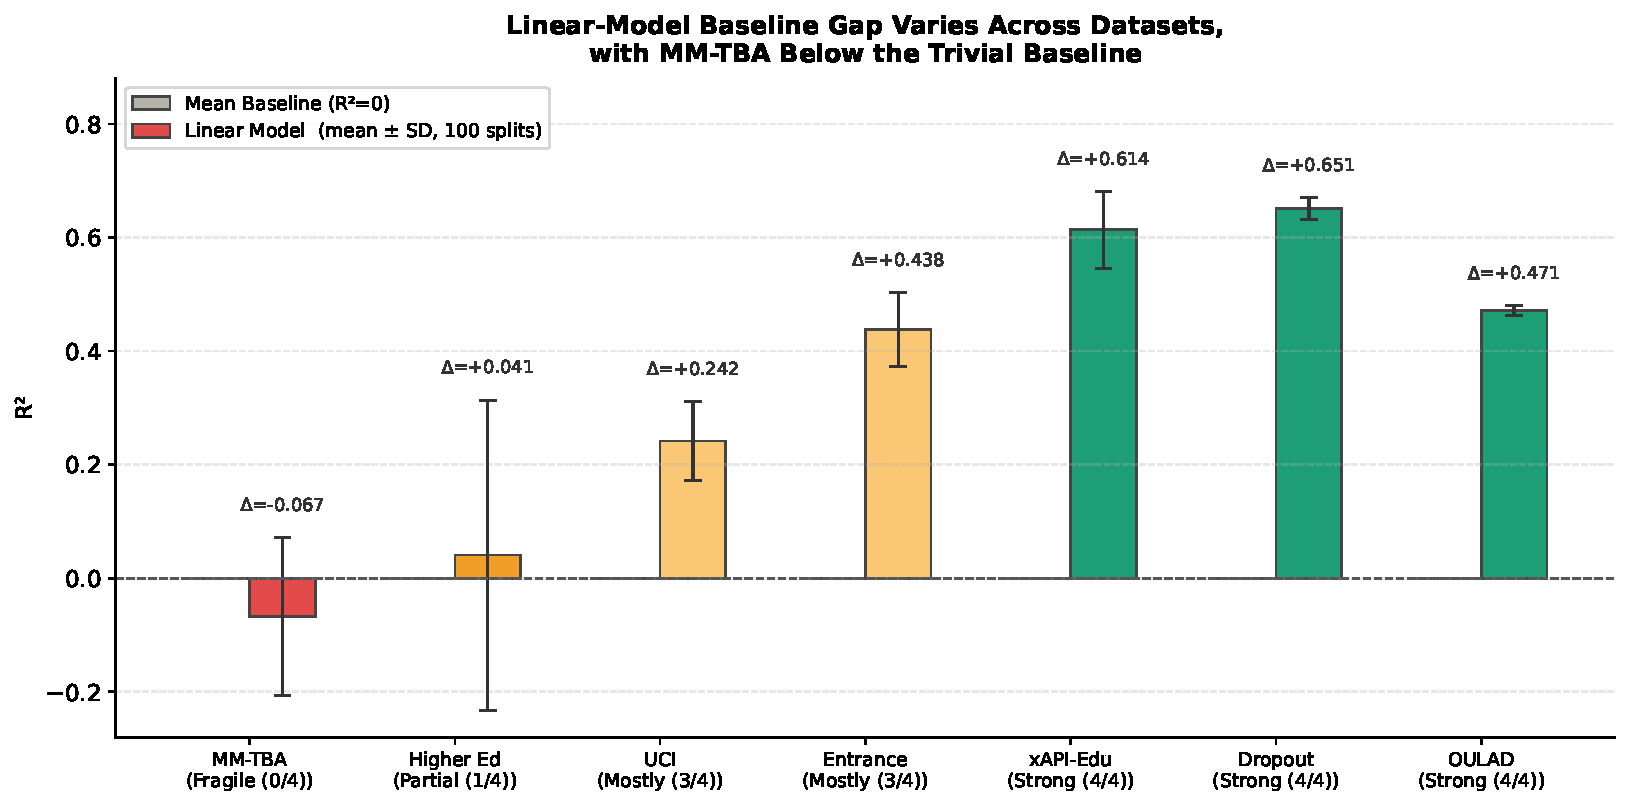
\includegraphics[width=0.95\textwidth]{../figures/figS1_baseline_gap.pdf}
\caption{Baseline gap: linear-model mean $R^2$ (with cross-split SD error bars) over 100 random 80/20 splits for the seven datasets, ordered by readiness profile. The grey reference bar denotes the trivial mean baseline ($R^2 = 0$). The figure complements Table~2 by showing the dispersion of split-level $R^2$ around the reported mean; MM-TBA and Higher~Ed have means near or below zero with relatively wide spread, consistent with their Fragile / Partial classifications.}
\label{fig:s_baseline_gap}
\end{figure}

\begin{figure}[!h]
\centering
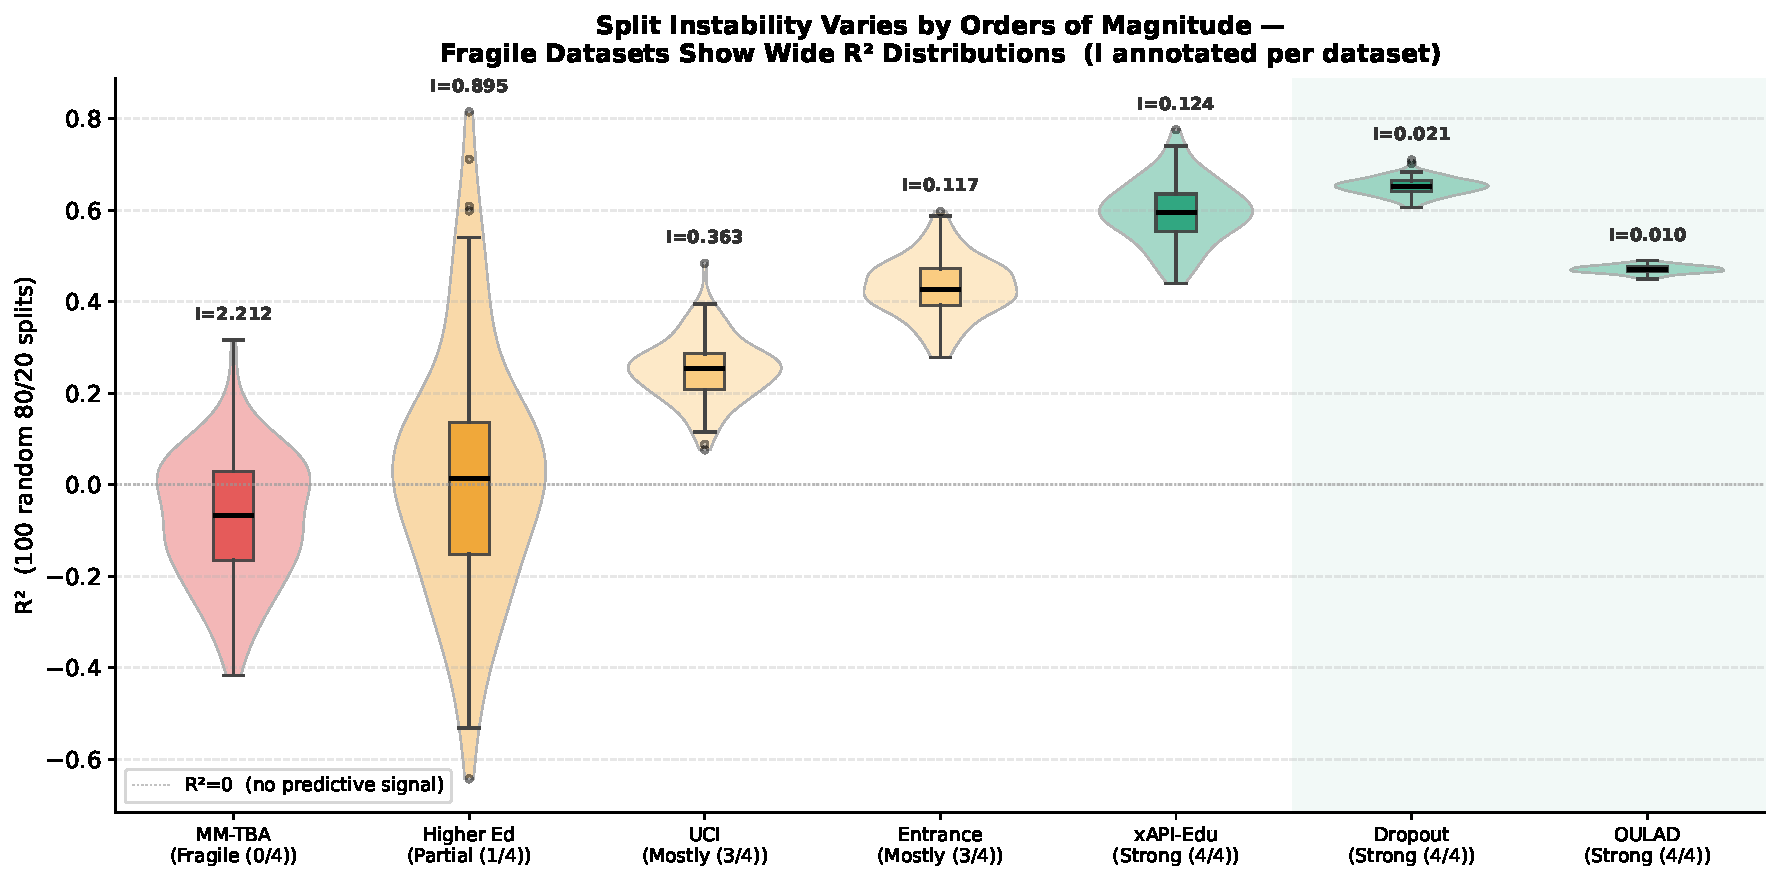
\includegraphics[width=0.95\textwidth]{../figures/figS2_split_instability.pdf}
\caption{Split instability: violin and box plots of the linear-model $R^2$ across 100 random 80/20 splits for each dataset, ordered by readiness profile. The instability ratio $I$ is annotated above each violin. Strong datasets (OULAD, Dropout) have tight distributions ($I < 0.03$); MM-TBA's distribution is broad and centred on negative $R^2$ ($I = 2.21$), reproducing Table~2 visually.}
\label{fig:s_split_instability}
\end{figure}

\begin{figure}[!h]
\centering
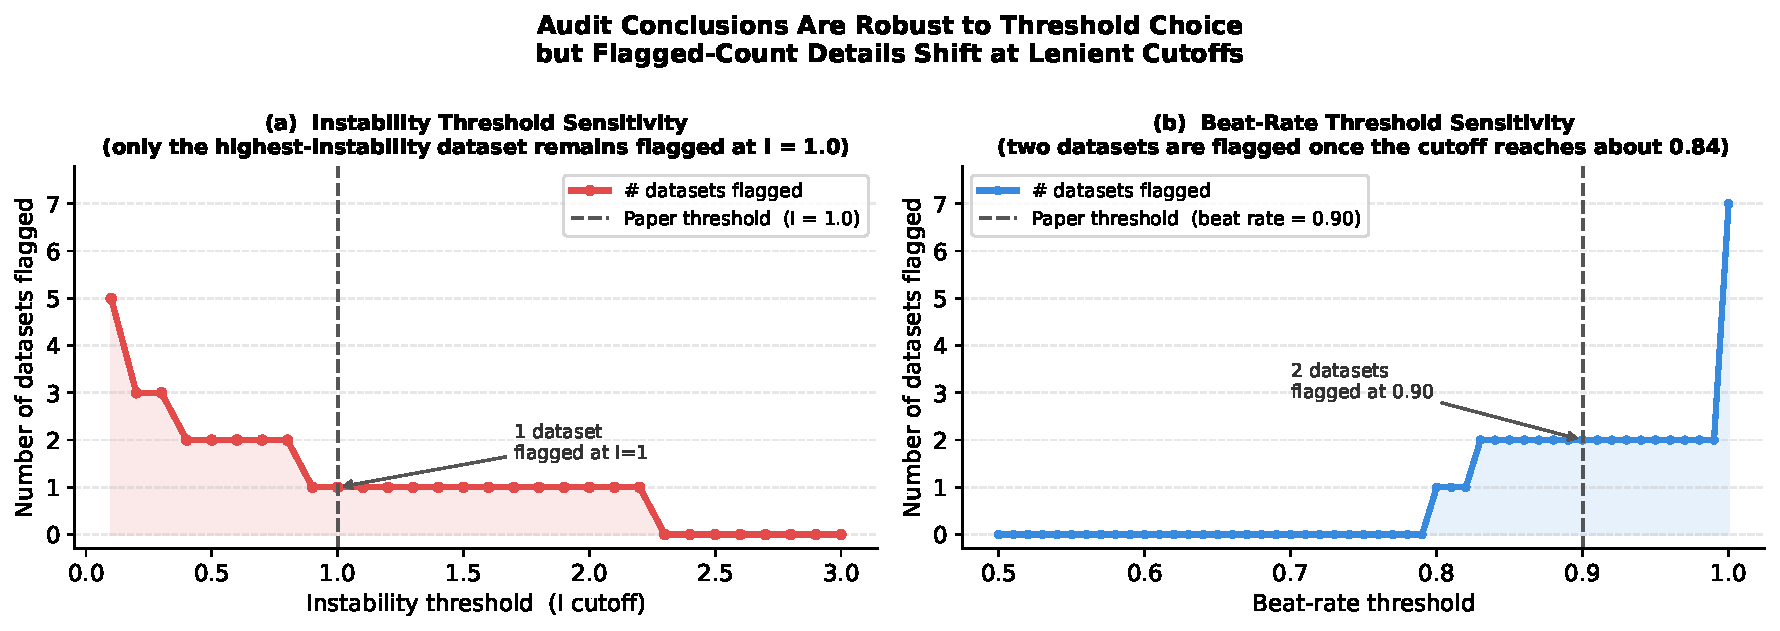
\includegraphics[width=0.95\textwidth]{../figures/figS3_threshold_sensitivity.pdf}
\caption{Threshold-sensitivity sweeps for the two operational cutoffs used in the audit. Panel~(a) varies the instability cutoff over $I \in [0.1, 3.0]$ and reports the number of datasets that would be flagged as failing split instability; the paper's choice of $I = 1.0$ flags one dataset (MM-TBA, with linear $I = 2.21$), while more lenient cutoffs below about $0.9$ additionally flag Higher~Ed. Panel~(b) varies the beat-rate cutoff over $[0.5, 1.0]$; the paper's choice of $0.90$ flags two datasets, whereas more lenient cutoffs below about $0.84$ reduce the flagged count. The main qualitative pattern remains unchanged: MM-TBA is always the weakest case, and Higher~Ed is the only borderline dataset near the operational thresholds.}
\label{fig:s_threshold_sensitivity}
\end{figure}

\end{document}
